% IDEA: separate theoretical/general approach and concrete decisions
% this means, for example, that:
% PART1:
% - requirements for lifted functions, soundness
% - implication (gradual, ...)
% - abstract versions of [w/o], append
% PART2:
% - concrete version of [w/o], append, ... (probably requires notion of normalized env :( )
% - actual implementation

\chapter{Introduction}
Most modern programming languages use static analysis to some degree, ruling out certain types of runtime failure.
Static analysis provides guarantees about the dynamic behavior of a program without actually running the program.
%% static typing
Static typing disciplines are among the most common representatives of static analysis, guaranteeing type safety at compile time, obviating the need for dynamic checks.

%% static verification
Another powerful technique is static verification of programs against their specification, i.e. statically proving their “correctness”.
In practice this is achieved by checking that some annotated invariants or assertions (reflecting the specification) must always hold.
% example?
Unfortunately, static verification has limitations and drawbacks:
\begin{itemize} % TODO
    \item Syntax
    \item Decidability
    \item Difficult and Tedious to annotate programs
    \item ...
\end{itemize}
These limitations not only affect programmers trying to statically verify their program.
Most general purpose programming languages (C/C++, C\#, Java, ...), usually driven by cost-benefit and usability considerations, haven't adopted this level of static analysis in the first place.

%% grad verification
The purpose of gradual verification is to weaken if not remove some of these limitations at the cost of turning some static checks into runtime checks, whenever inevitable.
We will present a procedure of turning a static verification into a gradual one.
% more detail about static limitations and how runtime circumvents them?

%% static typing weakened
This idea is not new at all and actually common practice in type systems:
In C\# or Java, explicit type casts are assertions about the actual type of a value.
This actual type (usually a subtype of the statically known type) could not be deduced by the static type system due to its limitations.
Such an assertion/cast allows subsequent static reasoning about the value assuming its new type at the cost of an additional runtime check, ensuring the validity of the cast.
Note that such deviations from a “purely” static type system (one where there is no need for runtime checks) do not affect type safety:
It is still guaranteed that execution does not enter an invalid state (one where runtime types are incompatible with statically annotated types) by simply interrupting execution whenever a runtime type check fails.
This is usually implemented by throwing an exception.
% mention that runtime cost reasonable, ...


%% dyn typing
At the other end of the spectrum are dynamically typed languages.
In scenarios where the limitations of a static type system would clutter up the source code, they allow expressing the same logic with less syntactic overhead, but at the cost of less static guarantees and early bug detection.

%% PLs are on the dynamic end of the verification spectrum
In terms of program verification, most general purpose languages are on the dynamic end of the spectrum.
If they exist as designated syntax, assertions are usually implemented as runtime checks and often even dropped entirely for “release” builds (the Java compiler drops them by default).
It is common practice to implement 
% research Eiffel!
% Design-by-Contract!!! Eiffel!
% D even has both

% this is more of a consequence of the “deep roots” of dynamic verification!!!
%But even preconditions at expression level are implemented as runtime checks, reflected all the way down at instruction architecture level.
%Examples:
%\begin{description}
%    \item[Division by zero]~\\
%    Integer division performs a dynamic check...
%    
%\end{description}

%% grad typing
A gradual type system is more flexible, as it provides the full continuum between static and dynamic typing, letting the programmer decide ... %TODO.
It can be seen as an extension  “unknown” type 


This work will also show that gradual verification ... other angle!

- 
What is the thesis about?
Why is it relevant or important?
What are the issues or problems?
What is the proposed solution or approach?
What can one expect in the rest of the thesis?


\chapter{Motivation}
more practical view? Intro? Background?


\chapter{Background and Motivation}

\section{Categorization of existing programming languages}

\section{Abstract Gradual Typing}

\section{Implicit Dynamic Frames}

\subsection{Self-Framing}

\section{Hoare Logic}
...for static semantics

\section{Motivation}
or here?


\chapter{Gradualization of a static... / A Statically Verified Language}
%% why start with static language
As illustrated earlier %MAKE SURE!
gradual verification can be seen as an extension of both static and dynamic verification.
% Both can be seen as the endpoints of the continuum...?
Yet, our approach of “gradualization” formalizes the introduction of the dynamic aspect into a fully static system.
Thus, this %TODO: work, section, chapter?
uses a statically verified language as starting point.
Later %TODO: ref
we will show how a programming language without static verification can be approached.

%% more about our language
We will now intrude a very simple Java-like language that uses Chalice/Eiffel/Spec\# %???
 sub-syntax to express method contracts.
% more about simplicity?

%% structure of this chapter
% TODO

\section{Syntax}
\label{sec:syntax}
Figure \ref{fig:idf-syntax} shows the full syntax of \svlidf.
\begin{figure}[h]
    \newcommand{\tempStmtA}{\sSkip
                    ~|~ \sDeclare {$T$} {$x$}
                    ~|~ \sFieldAssign {$x$} {$f$} {$y$} 
                    ~|~ \sVarAssign {$x$} {$e$}
                    ~|~ \sAlloc {$x$} {$C$} 
                    ~|~ \sCall {$x$} {$y$} {$m$} {$z$}}
\newcommand{\tempStmtB}{~~~ ~|~ \sReturn {$x$}  
                            ~|~ \sAssert {$\phi$} 
                            ~|~ \sRelease {$\phi$} 
                            ~|~ \sHold {$\phi$} {$s$}
                            ~|~ \sSeq {$s_1$} {$s_2$}}
\newcommand{\tempFrm}{  \phiTrue 
                    ~|~ \phiEq {$e$} {$e$} 
                    ~|~ \phiNeq {$e$} {$e$}
                    ~|~ \phiAcc {$e$} {$f$}
                    ~|~ \phiCons {$\phi$} {$\phi$}}
\newcommand{\tempExpr}{ \ev{$v$}
                    ~|~ \ex{$x$}
                    ~|~ \edot{$e$}{$f$}}

\begin{align*}
	program  & \in \setProgram    &  & ::= \ttt{$\overline{cls}$~$\overline{s}$}                         \\
	cls      & \in \setClass      &  & ::= \class {$C$} {$\overline{field}$} {$\overline{method}$}       \\
	field    & \in \setField      &  & ::= \field {$T$} {$f$}                                            \\
	method   & \in \setMethod     &  & ::= \method {$T$} {$m$} {$T$} {$x$} {$contract$} {$\overline{s}$} \\
	contract & \in \setContract   &  & ::= \ttt{requires $\phi$;~ensures $\phi$;}                        \\
	T        & \in \setType       &  & ::= \Tint ~|~ C                                                   \\
	s        & \in \setStmt       &  & ::= \tempStmtA                                                    \\
	         &                    &  & \tempStmtB                                                        \\
	\phi     & \in \setFormula    &  & ::= \tempFrm                                                      \\
	e        & \in \setExpr       &  & ::= \tempExpr                                                     \\
	x, y, z  & \in \setVar        &  & ::= \ethis ~|~ \eresult ~|~ name                                  \\
	v        & \in \setVal        &  & ::= o ~|~ n ~|~ \enull                                            \\
	o        & \in \setObj        &  &  \\
	n        & \in \mathbb{Z}     &  &  \\
	C        & \in \setClassName  &  & ::= name                                                          \\
	f        & \in \setFieldName  &  & ::= name                                                          \\
	m        & \in \setMethodName &  & ::= name
\end{align*} 
    \caption{\svlidf: Syntax}
    \label{fig:idf-syntax}
\end{figure}
% EXPLAIN what stuff (like hold, release) means!

%% parser rassoc, skip
\FloatBarrier
We define $\ttt{;}$ to be right-associative and assume that parsing a sequence of statements (e.g. method body) operates analogously, obviating the need for parenthesis.
Furthermore we assume that the parser terminates every sequence with $\sSkip$.
\begin{exmp}~
    \begin{lstlisting}
    ...
    {
        $s_1$;
        $s_2$;
        $s_3$;
    }
    \end{lstlisting}
    is parsed as
    
    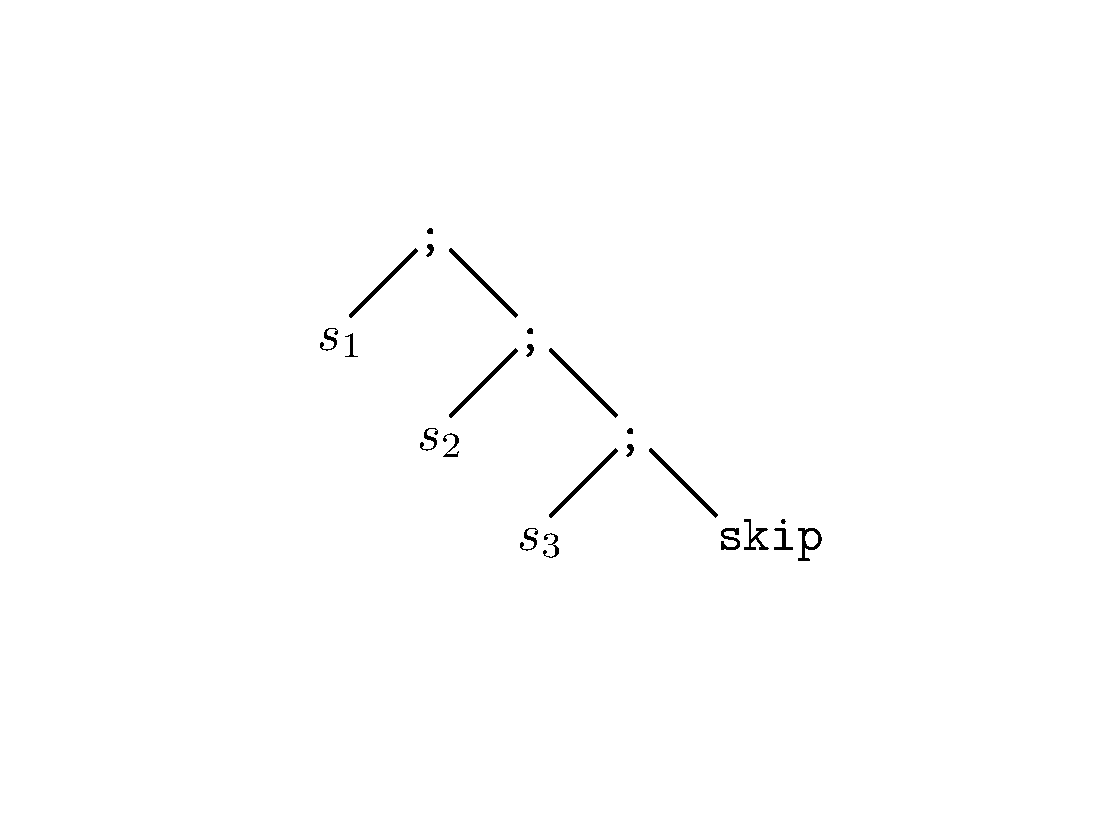
\includegraphics[trim={3cm 3cm 3cm 3cm}, clip, width=6cm]{graphics/rightAssocSkip}
\end{exmp}
These assumptions highly simplify reasoning about statements.


\section{Static Semantics}
\label{sec:static-semantics}
% AXIOMATIC
The static semantics of \svl consist of typing rules and a Hoare calculus making use of those typing rules.
All the rules are implicitly parameterized over some program $p \in \setProgram$, necessary for example to extract the type of a field in the following typing rules.

\begin{figure}[h]
    \boxed{\sType{\Gamma}{e}{T}}
    %% Inductive Semantics.hasStaticType
\begin{mathpar}
\inferrule* [Right=STValNum]
{
    ~
}
{
    \sType {\Gamma} {\ev{${{n}}$}} {\Tint}
}
\end{mathpar}

\begin{mathpar}
\inferrule* [Right=STValNull]
{
    ~
}
{
    \sType {\Gamma} {\ev{${\enull}$}} {{C}}
}
\end{mathpar}

\begin{mathpar}
\inferrule* [Right=STVar]
{
    {\Gamma(x)} = {{T}}
}
{
    \sType {\Gamma} {\ex{${x}$}} {T}
}
\end{mathpar}

\begin{mathpar}
\inferrule* [Right=STField]
{
    \sType {\Gamma} {e} {{C}} \\
    {\fieldType({C}, {f})} = {{T}}
}
{
    \sType {\Gamma} {\edot{${e}$}{${f}$}} {T}
}
\end{mathpar}


% Inductive Semantics.hasStaticType
\begin{mathpar}
\inferrule* [right=STValNum]
{
    ~
}
{
    \sType {\Gamma} {\ev{${{n}}$}} {\Tint}
}

\inferrule* [right=STValNull]
{
    ~
}
{
    \sType {\Gamma} {\ev{${\enull}$}} {{C}}
}

\inferrule* [right=STVar]
{
    {\Gamma(x)} = {{T}}
}
{
    \sType {\Gamma} {\ex{${x}$}} {T}
}

\inferrule* [right=STField]
{
    \sType {\Gamma} {e} {{C}} \\
    {\fieldType({C}, {f})} = {{T}}
}
{
    \sType {\Gamma} {\edot{${e}$}{${f}$}} {T}
}
\end{mathpar}


    \caption{\svl: Static Typing of Expressions}
\end{figure}

\begin{figure}[h!]
    \boxed{\thoare {\Gamma} {\phi_{pre}} {\overline{s}} {\phi_{post}}}
    % Inductive Semantics.hoare
\begin{mathpar}
\inferrule* [Right=HAlloc]
{
    {\phi} \implies {\phi'} \\
    {\emptyset} \sfrmphi {\phi'} \\
    {x} \not \in {FV(\phi')} \\
    {\Gamma} \vdash {\ex{${x}$}} : {{C}} \\
    {\fields({C})} = {{\overline{f}}}
}
{
    {\Gamma} \hoare {\phi} {{\sAlloc {${x}$} {${C}$}}} {\phiCons{${\phi'}$}{${\phiCons{${\phiNeq {${\ex{${x}$}}$} {${\ev{${\vnull}$}}$}}$}{${\overline{\acc({x}, f_i)}}$}}$}}
}
\end{mathpar}

\begin{mathpar}
\inferrule* [Right=HFieldAssign]
{
    {\phi} \implies {\phiCons{${\phiAcc {${\ex{${x}$}}$} {${f}$}}$}{${\phi'}$}} \\
    {\emptyset} \sfrmphi {\phi'} \\
    {\Gamma} \vdash {\ex{${x}$}} : {{C}} \\
    {\Gamma} \vdash {\ex{${y}$}} : {T} \\
    \vdash {C}.{f} : {T}
}
{
    {\Gamma} \hoare {\phi} {{\sFieldAssign {${x}$} {${f}$} {${y}$}}} {\phiCons{${\phi'}$}{${\phiCons{${\phiAcc {${\ex{${x}$}}$} {${f}$}}$}{${\phiCons{${\phiNeq {${\ex{${x}$}}$} {${\ev{${\vnull}$}}$}}$}{${\ensuremath{{\phiEq {${\edot{${\ex{${x}$}}$}{${f}$}}$} {${\ex{${y}$}}$}}}}$}}$}}$}}
}
\end{mathpar}

\begin{mathpar}
\inferrule* [Right=HVarAssign]
{
    {\phi} \implies {\phi'} \\
    {\emptyset} \sfrmphi {\phi'} \\
    {x} \not \in {FV(\phi')} \\
    {x} \not \in {FV({e})} \\
    {\Gamma} \vdash {\ex{${x}$}} : {T} \\
    {\Gamma} \vdash {e} : {T} \\
    {\accFor {{e}}} \subseteq {\phi'}
}
{
    {\Gamma} \hoare {\phi} {{\sVarAssign {${x}$} {${e}$}}} {\phiCons{${\phi'}$}{${\ensuremath{{\phiEq {${\ex{${x}$}}$} {${e}$}}}}$}}
}
\end{mathpar}

\begin{mathpar}
\inferrule* [Right=HReturn]
{
    {\phi} \implies {\phi'} \\
    {\emptyset} \sfrmphi {\phi'} \\
    {\xresult} \not \in {FV(\phi')} \\
    {\Gamma} \vdash {\ex{${x}$}} : {T} \\
    {\Gamma} \vdash {\ex{${\xresult}$}} : {T}
}
{
    {\Gamma} \hoare {\phi} {{\sReturn {${x}$}}} {\phiCons{${\phi'}$}{${\ensuremath{{\phiEq {${\ex{${\xresult}$}}$} {${\ex{${x}$}}$}}}}$}}
}
\end{mathpar}

\begin{mathpar}
\inferrule* [Right=HCall]
{
    {\Gamma} \vdash {\ex{${y}$}} : {{C}} \\
    {\mmethod({C}, {m})} = {{\method {${T_r}$} {${m}$} {${T_p}$} {${z}$} {${\requires {\phi_{pre}};~\ensures {\phi_{post}};}$} {${\_}$}}} \\
    {\Gamma} \vdash {\ex{${x}$}} : {T_r} \\
    {\Gamma} \vdash {\ex{${z'}$}} : {T_p} \\
    {\phi} \implies {\phiCons{${\phiNeq {${\ex{${y}$}}$} {${\ev{${\vnull}$}}$}}$}{${\phiCons{${\phi_p}$}{${\phi'}$}}$}} \\
    {\emptyset} \sfrmphi {\phi'} \\
    {x} \not \in {FV(\phi')} \\
    x \neq y \wedge x \neq z' \\
    {\phi_p} = {{\phi_{pre}}[{y}, {z'} / {\xthis}, {{z}}]} \\
    {\phi_q} = {{\phi_{post}}[{y}, {z'}, {x} / {\xthis}, {{z}}, {\xresult}]}
}
{
    {\Gamma} \hoare {\phi} {{\sCall {${x}$} {${y}$} {${m}$} {${z'}$}}} {\phiCons{${\phi'}$}{${\phi_q}$}}
}
\end{mathpar}

\begin{mathpar}
\inferrule* [Right=HAssert]
{
    {\phi} \implies {\phi'}
}
{
    {\Gamma} \hoare {\phi} {{\sAssert {${\phi'}$}}} {\phi}
}
\end{mathpar}

\begin{mathpar}
\inferrule* [Right=HRelease]
{
    {\phi} \implies {\phiCons{${\phi_r}$}{${\phi'}$}} \\
    {\emptyset} \sfrmphi {\phi'}
}
{
    {\Gamma} \hoare {\phi} {{\sRelease {${\phi_r}$}}} {\phi'}
}
\end{mathpar}

\begin{mathpar}
\inferrule* [Right=HDeclare]
{
    {x} \not\in \dom({\Gamma}) \\
    {{\Gamma}, {x} : {T}} \hoare {\phiCons{${\phiEq {${\ex{${x}$}}$} {${\ev{${\texttt{defaultValue}({T})}$}}$}}$}{${\phi}$}} {\overline{s}} {\phi'}
}
{
    {\Gamma} \hoare {\phi} {{\sDeclare {${T}$} {${x}$}} {\overline{s}}} {\phi'}
}
\end{mathpar}

\begin{mathpar}
\inferrule* [Right=HHold]
{
    {\phi_f} \implies {\phiCons{${\phi_r}$}{${\phi'}$}} \\
    {\phi'} \implies {\phi} \\
    {\Gamma} \hoare {\phi_r} {\overline{s}} {\phi_r'}
}
{
    {\Gamma} \hoare {\phi_f} {{\sHold {${\phi}$} {${\overline{s}}$}}} {\phiCons{${\phi_r'}$}{${\phi'}$}}
}
\end{mathpar}

\begin{mathpar}
\inferrule* [Right=HSeq]
{
    {\Gamma} \hoare {\phi_p} {\overline{s_1}} {\phi_q} \\
    {\Gamma} \hoare {\phi_q} {\overline{s_2}} {\phi_r}
}
{
    {\Gamma} \hoare {\phi_p} {{\overline{s_1}}\ttt{;} {\overline{s_2}}} {\phi_r}
}
\end{mathpar}


    \caption{\svl: Hoare Calculus} 
\end{figure}


%% FRAMING
%% Inductive Semantics.sfrme
\begin{mathpar}
\inferrule* [Right=WFVar]
{
    ~
}
{
    {A} \sfrme {\ex{${x}$}}
}
\end{mathpar}

\begin{mathpar}
\inferrule* [Right=WFValue]
{
    ~
}
{
    {A} \sfrme {\ev{${v}$}}
}
\end{mathpar}

\begin{mathpar}
\inferrule* [Right=WFField]
{
    {({e}, {f})} \in {A} \\
    {A} \sfrme {e}
}
{
    {A} \sfrme {\edot{${e}$}{${f}$}}
}
\end{mathpar}



\section{Well-Formedness}
\label{sec:well-formedness}
Apart from checking method contracts, a verifier or compiler may enforce further rules before accepting a program as “well formed”.
For \svlidf we give the rules formalized in figure \ref{fig:idf-wf}.

\begin{figure}[h]
    
\begin{mathpar}
\inferrule* [Right=OkProgram]
{
\overline{cls_i \OK} \\
\thoare {~} {\phiTrue} {s} {\phi}
}
{(\overline{cls_i}~s) \OK}
\end{mathpar}

\begin{mathpar}
\inferrule* [Right=OkClass]
{
\text{unique $field$-names} \\
\text{unique $method$-names} \\
\overline{method_i \OKinC}
}
{(\class {$C$} {$\overline{field_i}$} {$\overline{method_i}$}) \OK}
\end{mathpar}

\begin{mathpar}
\inferrule* [Right=OkMethod]
{
    \thoare {x : T_x, \ethis : C, \eresult : T_m} {\phi_1} {s} {\phi_2} \\\\
    \FV(\phi_1) \subseteq \{ x, \ethis \} \\
    \FV(\phi_2) \subseteq \{ x, \ethis, \eresult \} \\\\
    \sfrmphi \phi_1 \\
    \sfrmphi \phi_2 \\
    \neg \writesTo(s, x)
}
{(\method {$T_m$} {$m$} {$T_x$} {$x$} {\contract {$\phi_1$} {$\phi_2$}} {$s$}) \OKinC}
\end{mathpar}
    \caption{\svlidf: Well-Formedness}
    \label{fig:idf-wf}
\end{figure}

%% OkMethod
The premises of $\tset{OkMethod}$ make sure that reasoning about calls is sound.
As expected, the method contract is checked, while also making sure that it contains self-framing formulas.
Furthermore, the free variables are restricted to those occurring in the method signature.
The following example illustrates why this is necessary.

%% example
\begin{example}{Leaking Postcondition}
\begin{lstlisting}
int identity(int a)
    requires true;
    ensures  (b = 3);
{
    int b;
    b = 3;
    return a;
}
\end{lstlisting}
While the method passes static verification, it could lead to unsound proofs.
Note how \tset{HCall} forwards the postcondition after replacing known variables with their counterparts.
\phiEq{b}{3} is unaffected by this replacement, ending up in the postcondition of the call statement.

Should the call site also know a variable \ttt{b}, then \phiEq{b}{3} will most likely not reflect the state of that variable.
\end{example}

For similar reasons, we prevent writes to the method's parameter.
Changes to the parameter would otherwise end up in the postcondition which is forwarded to the call site.
Information about the formal parameter is then reflected back on the variable passed as actual parameter for the method call.
However, since parameters are passed by value, this information would be false -- the actual parameter will have the same value before and after the method call.


\section{Dynamic Semantics}



\chapter{Deriving a Gradual Language}

\section{Abstracting Static Semantics}

\section{Abstracting Dynamic Semantics}


\chapter{Implementation}


\chapter{Evaluation/Analysis}



\chapter{Conclusion}
Recap, remind reader what big picture was.
Briefly outline your thesis, motivation, problem, and proposed solution.

\section{Limitations}

\section{Future Work}


\chapter{Appendix}


\chapter{UNSORTED}

\section{HoareMotivEx}
\label{sec:hoaremotivex}

% AGT: mention draft about refinement types?

Hoare Logic as formal setting

\begin{verbatim}
class Point
{
    int manhattenDistance(Point p)
        requires \phi_{pre};
        ensures  \phi_{post};
    {
        s1;
        s2;
        .
        .
        .
    }
}
\end{verbatim}

\begin{displaymath}
\thoare
    {\ethis : \type{Point}, \ex{p} : \type{Point}, \eresult : \Tint}
    {\phi_{pre}}
    {s1; s2; ...}
    {\phi_{post}}
\end{displaymath}

\section{MotivationExamples}
\label{sec:motivationexamples}

\subsection{Argument Validation}
The following Java example motivates the use of verification for argument validation.
\begin{lstlisting}
boolean hasLegalDriver(Car c)
{
    // business logic:
    resAllocate();
    boolean result = c.driver.age >= 18;
    resFree();
    return result;
}
\end{lstlisting}
A call to \ttt{hasLegalDriver} fails if \ttt{c} or \ttt{c.driver} evaluate to \ttt{null}.
Note that, although the Java runtime has defined behavior in to those cases (throwing an exception), we might still have created a resource leak.
To prevent this from happening, arguments have to be validated before entering the business logic.
\begin{lstlisting}
boolean hasLegalDriver(Car c)
{
    if (!(c != null))
        throw new IllegalArgException("expected c != null");
    if (!(c.driver != null))
        throw new IllegalArgException("expected c.driver != null");
        
    // business logic (requires 'c.driver.age' to evaluate)
}
\end{lstlisting}

Note that these runtime checks dynamically verifies a method contract, having \ttt{c != null \&\& c.driver != null} as precondition.
Naturally, the drawbacks of dynamic verification apply:
Violations of the method contract are only detected at runtime, possibly go unnoticed for a long time and impose a runtime overhead which might not be acceptable in all scenarios.
Java even has dedicated assertion syntax simplifying dynamic verification:
\begin{lstlisting}
boolean hasLegalDriver(Car c)
{
    assert c != null;
    assert c.driver != null;

    // business logic (requires 'c.driver.age' to evaluate)
}
\end{lstlisting}
Note however that such assertions are dropped from regular builds, meaning that the method contract is no longer verified!

With support of additional tools, a more declarative approach is possible using JML syntax:
\begin{lstlisting}
//@ requires c != null && c.driver != null;
boolean hasLegalDriver(Car c)
{
    // business logic (requires 'c.driver.age' to evaluate)
}
\end{lstlisting}

There are two basic ways to turn this annotation into a guarantee:
\begin{description}
    \item[Static Verification (e.g. ESC/Java, see \cite{leino2000esc})]~\\
    Verification will only succeed if the precondition is provable at all call sites.
    This is achievable in two ways:
    \begin{itemize}
        \item
        Rigorously annotate the call sites, guiding the verifier towards a proof.
        \item 
        Add parameter validation to the call sites, effectively duplicating the original runtime check across the program.
        Note that this approach combines static and dynamic validation in order to get a performance benefit (no more runtime checks required where precondition was provable) and circumvent rigorous annotation.
        The drawback is of course code duplication.
    \end{itemize}
    % benefits, drawbacks
    
    %There are obvious limitations to this approach, static verification tends to be invasive.
    %At least there is a performance benefit: 
    %Runtime checks (originally part of every call) are now only necessary in places where verification would not succeed otherwise.
    
    \item[Dynamic Verification (e.g. run JML4c, see \cite{sarcar2010new}]~\\
    This approach basically converts the annotation back into a runtime check equivalent to our original argument validation.
    % benefits, drawbacks
\end{description}

Gradual verification would pursue the combined approach without (visible) code duplication:
Static verification is used where possible, dynamic verification where needed.
Note that for the programmer this means that adding the method contract comes with no further obligations.

\subsection{Limitations of Static Verification}
The following example is written in a Java-like language with dedicated syntax for method contracts (similar to Eiffel and Spec\#).
We assume that this language is statically verified, i.e. static verification is part of the compilation.

The example shows the limitations of static verification using the Collatz sequence as an algorithm too complex to describe concisely in a method contract:
\begin{lstlisting}
int collatzIterations(int iter, int start)
    requires 1 <= start;
    ensures  1 <= result;
{
    // ...
}

int myRandom(int seed)
    requires 1 <= seed   && seed   <= 10000;
    ensures  1 <= result && result <= 3;     // not provable
{
    int result = collatzIterations(300, seed);
    // we know:        result $\in$ { 1, 2, 4 }
    // verifier knows: 1 <= result
    
    if (result == 4) result = 3;
    return result;
}
\end{lstlisting}
The first method \ttt{collatzIterations} iterates given number of times, starting at given value.
We assume that the only provable contract is that positive start value results in positive result.
The second method \ttt{myRandom} uses the Collatz sequence to generate a pseudo random number from given seed.
It is known to the programmer that start values up to 10000 result in convergence of the sequence after 300 iterations.
After mapping 4 to 3, we are thus given a number between 1 and 3, as described in the postcondition.

Unfortunately, the verifier cannot deduce this fact since the postcondition of \ttt{collatzIterations} only guarantees positive result, but no specific range of values.
Again, we can resort to dynamic methods to aid verification:

\begin{lstlisting}
...
{
    int result = collatzIterations(300, seed);
    // we know:        result $\in$ { 1, 2, 4 }
    // verifier knows: 1 <= result
    
    // knowledge "cast"
    if (!(result <= 4))
        throw new IllegalStateException("expected result <= 4");

    // verifier knows: 1 <= result && result <= 4 
    
    if (result == 4) result = 3;
    return result;
}
\end{lstlisting}

This solution is not satisfying as it required additional work by the programmer to convince the verifier.
Furthermore, the solution is in an unintuitive location:
The problem is not caused by \ttt{myRandom}, yet it is solved there.
The actual problem is that the postcondition of \ttt{collatzIterations} is too weak, causing the verifier to fail deducing our knowledge.

Gradual verification allows enhancing the postcondition with “unknown” knowledge that can be reinterpreted arbitrarily, adding appropriate runtime checks to guarantee that this reinterpretation was in fact valid:
\begin{lstlisting}
int collatzIterations(int iter, int start)
    requires 1 <= start;
    ensures  1 <= result && ?;
{
    // ...
}

int myRandom(int seed)
    requires 1 <= seed   && seed   <= 10000;
    ensures  1 <= result && result <= 3;
{
    int result = collatzIterations(300, seed);
    // we know: result $\in$ { 1, 2, 4 }
    
    // verifier allowed to
    //  assume 1 <= start && result <= 4
    //  from   1 <= start && ?
    // (adding runtime check)
    
    if (result == 4) result = 3;
    return result;
}
\end{lstlisting}
Note the \ttt{?} in the postcondition of \ttt{collatzIterations}.

% gradual:
% - not in a sense of GraVy
% - assertions are GUARANTEED not to be violated (analogous to type safety of gradually typed languages), meaning that
%    - as much as possible is verified statically
%    - if necessary, (ideally: as few as possible) dynamic checks kick in
% - full continuum between static and dynamic

% static checking
% dynamic checking
% combine static and dynamic checking
% views:
% - add designated "?" to statically checked language, making checking optional
% - introduce checking to unchecked language, making "?" the default value
% typing
% transition to verification
% - of particular interest, cause limitations due to syntax or decidability make full checking impossible,
%    possibly making use of static verification impossible and the program thus unverifiable
%    inevitable incompleteness of static verifiers!
%    GraVy: measure, only \textit{classifies} code into sections: correctness statically guaranteed, correctness statically disproved, no static guarantee so far

% very desirable in practice
% gradual version of a language is inherently a strict superset of original language
% 

% our approach allows extension of existing languages (without any verification) by adding transpilation step

% why would you want continuum?
% - move toward satically verified program without giving up guarantees!
% - while "barely typed" languages hardly make sense, programs with "little verification" are already highly useful
%    i.e. verification even makes sense as "rarely used feature"!
%    ArgumentException-example
%    -    performance benefit!
%    -    cleaner code!
%    -    makes more sense semantically
% having optional types 

% Future Work:
% implement on top of existing languages
% - tracking access via ThreadLocalStorage
% - transpilation (e.g. C# Roslyn compiler extension)
